%%%%%%%% ICML 2026 EXAMPLE LATEX SUBMISSION FILE %%%%%%%%%%%%%%%%%

\documentclass{article}

% Recommended, but optional, packages for figures and better typesetting:
\usepackage{microtype}
\usepackage{graphicx}
\usepackage{subcaption}
\usepackage{booktabs} % for professional tables

% hyperref makes hyperlinks in the resulting PDF.
% If your build breaks (sometimes temporarily if a hyperlink spans a page)
% please comment out the following usepackage line and replace
% \usepackage{icml2026} with \usepackage[nohyperref]{icml2026} above.
\usepackage{hyperref}
\usepackage{float}
\graphicspath{{figures/}} % Location of the graphics files


% Attempt to make hyperref and algorithmic work together better:
\newcommand{\theHalgorithm}{\arabic{algorithm}}

% Use the following line for the initial blind version submitted for review:
\usepackage{icml2026}

% For preprint, use
% \usepackage[preprint]{icml2026}

% If accepted, instead use the following line for the camera-ready submission:
% \usepackage[accepted]{icml2026}

\usepackage{amsmath}
\usepackage{amssymb}
\usepackage{mathtools}
\usepackage{amsthm}


% if you use cleveref..
\usepackage[capitalize,noabbrev]{cleveref}

%%%%%%%%%%%%%%%%%%%%%%%%%%%%%%%%
% THEOREMS
%%%%%%%%%%%%%%%%%%%%%%%%%%%%%%%%
\theoremstyle{plain}
\newtheorem{theorem}{Theorem}[section]
\newtheorem{proposition}[theorem]{Proposition}
\newtheorem{lemma}[theorem]{Lemma}
\newtheorem{corollary}[theorem]{Corollary}
\theoremstyle{definition}
\newtheorem{definition}[theorem]{Definition}
\newtheorem{assumption}[theorem]{Assumption}
\theoremstyle{remark}
\newtheorem{remark}[theorem]{Remark}

% Todonotes is useful during development; simply uncomment the next line
%    and comment out the line below the next line to turn off comments
%\usepackage[disable,textsize=tiny]{todonotes}
\usepackage[textsize=tiny]{todonotes}
\usepackage{xcolor}
\usepackage{booktabs}
% Mark new additions in blue.  Use {\color{blue}...} for multi-paragraph blocks.
\newcommand{\new}[1]{{\color{blue}#1}}

% The \icmltitle you define below is probably too long as a header.
% Therefore, a short form for the running title is supplied here:
\icmltitlerunning{Physics Informed Neural Networks with Learnable Scaling for Feature Engineering}

\begin{document}

\twocolumn[
  \icmltitle{Physics Informed Neural Networks with Learnable Scaling for Feature Engineering}

  % It is OKAY to include author information, even for blind submissions: the
  % style file will automatically remove it for you unless you've provided
  % the [accepted] option to the icml2026 package.

  % List of affiliations: The first argument should be a (short) identifier you
  % will use later to specify author affiliations Academic affiliations
  % should list Department, University, City, Region, Country Industry
  % affiliations should list Company, City, Region, Country

  % You can specify symbols, otherwise they are numbered in order. Ideally, you
  % should not use this facility. Affiliations will be numbered in order of
  % appearance and this is the preferred way.
  \icmlsetsymbol{equal}{*}

  \begin{icmlauthorlist}
    \icmlauthor{Varvara Nazarenko}{equal,HSE}
    \icmlauthor{Alexander Tarakanov}{equal,HSE, VK}
  \end{icmlauthorlist}

  \icmlaffiliation{HSE}{Faculty of Computer Science, Higher School of Economics, Moscow, Russia}
  \icmlaffiliation{VK}{VK, Moscow, RUssia}
  

  \icmlcorrespondingauthor{Varvara Nazarenko}{varunaza@gmail.com}
  \icmlcorrespondingauthor{Alexander Tarakanov}{atarakanov@hse.ru}

  % You may provide any keywords that you find helpful for describing your
  % paper; these are used to populate the "keywords" metadata in the PDF but
  % will not be shown in the document
  \icmlkeywords{Machine Learning, Physics Informed Neural Networks, Feature Engineering, ICML}

  \vskip 0.3in
]

% this must go after the closing bracket ] following \twocolumn[ ...

% This command actually creates the footnote in the first column listing the
% affiliations and the copyright notice. The command takes one argument, which
% is text to display at the start of the footnote. The \icmlEqualContribution
% command is standard text for equal contribution. Remove it (just {}) if you
% do not need this facility.

% Use ONE of the following lines. DO NOT remove the command.
% If you have no special notice, KEEP empty braces:
\printAffiliationsAndNotice{}  % no special notice (required even if empty)
% Or, if applicable, use the standard equal contribution text:
% \printAffiliationsAndNotice{\icmlEqualContribution}

\begin{abstract}

Spectral methods are widely used in machine learning for feature engineering and representation learning. Typically, such approaches rely on defining a kernel or an integral/differential operator whose eigenfunctions are then used to construct data-driven features. In practice, however, the performance of spectral methods is highly sensitive to the choice of kernel, feature scaling, and associated hyperparameters, often requiring substantial manual tuning.

In this work, we propose an alternative spectral framework that alleviates these limitations. Our approach is based on eigenfunctions of a modified Dirichlet energy functional, defined as the expected squared norm of the gradient of a function. The key modification consists in introducing a learnable linear transformation of the gradient within the Dirichlet energy, allowing the spectral structure to be adapted directly from data.

This formulation provides several important benefits. First, it relaxes the classical manifold hypothesis by interpolating between differential-geometric operators, such as the Laplace–Beltrami operator, and purely statistical objects defined by energy spectra. Second, it significantly reduces the need for manual hyperparameter tuning and feature scaling, as the relevant transformations are learned automatically. Finally, the proposed method yields compact and expressive data representations that are naturally aligned with downstream tasks, such as classification.

\new{We empirically validate the proposed approach on six benchmark datasets spanning binary and multi-class classification:
Two Moons, Circles, HTRU2, MNIST, Fashion-MNIST, and CIFAR-10.
The EFDO method with diagonal metric achieves \(94.53\%\) validation accuracy on MNIST and \(85.50\%\) on CIFAR-10 features, surpassing the NeuralEF baseline~\citep{pmlr-v162-deng22b} by \(+12.0\) pp and \(+9.4\) pp respectively (NeuralEF: \(82.52\%\) / \(76.05\%\), \(K{=}16\) eigenfunctions).
Training curves and learned eigenfunction visualisations confirm stable convergence and meaningful geometric structure.}

\end{abstract}

\section{Introduction}

\paragraph{Contributions.}
The main contributions of this work are as follows:
\begin{itemize}
\item We introduce a learnable modification of the Dirichlet energy that generalizes classical spectral operators.
\item We show that the resulting eigenfunctions provide compact and task-adaptive representations.
\item We demonstrate empirically that the proposed approach reduces sensitivity to feature scaling and hyperparameter tuning.
\new{\item We evaluate the approach on \textbf{six benchmarks} (Two Moons, Circles, HTRU2, MNIST, Fashion-MNIST, CIFAR-10) and compare against Random Forest, Logistic Regression, and NeuralEF baselines.
\item We introduce and compare three metric parametrisations—identity (\textsc{off}), diagonal (\textsc{diag}), and Trotter-product rotation (\textsc{trotter})—analysing their effect on representation quality.}
\end{itemize}

\label{sec:introduction}
Artificial Neural Networks (ANN) \citet{rosenblatt1958perceptron} are routinely utilized to solve real-world problems:
medical image segmentation \citet{ajmal2018convolutional}, 
medical diagnostics \citet{amato2013artificial}, photo and video processing and enhancement \citet{ahmadi2016unsupervised},
face recognition \citet{le2011applying}, text processing \citet{chang2023survey} etc.
It has been shown in recent decades that ANN can handle such problems as numerical solution for PDEs
and for calculation of differential and integral operators eigenfunctions \citet{Jin2020UnsupervisedNN}.
In the current work we propose a novel approach for calculation of the Dirichlet Energy \citet{evans2022partial} eigenfunctions.


The main motivation for this work is provided by Graph-Laplacian methods \citet{4476091}.
In this family of methods the graph is constructed based on the available data and
the spectrum of Laplacian associated with this graph is computed \citet{10.1137/1.9781611972801.49}.
Eigen-functions of that Laplace operator have extremely useful properties especially when data is sampled from a certain manifold.
First of all, it can be shown that the number of components of the graph 
is greater or equal to the dimension of Laplace operator kernel \citet{BELKIN20081289}.
This fact gives rise to a variety of clustering algorithms 
including the well-known spectral clustering method \citet{NIPS2001_801272ee}.
In addition to that, eigenfunctions of the Laplacian allows one to perform Fourier analysis
in the space of functions on the graph vertices \citet{kostopoulos2018semi}
The latter gives rise to the variety of algorithms for semi-supervised learning \citet{sheikhpour2018semi}..
In other words, eigenfunctions of Laplace operator on Graph can be successfully utilized to propagate labels from few labeled samples
to the entire dataset \citet{646eb8ee0f50464f8db1e953d2df93c3}.


The reason for such remarkable performance is that eigenfunctions of Laplace operator on the graph converge to the eigenfunctions
of Laplace-Beltrami operator if data is sampled from the manifold as it has been shown in the pioneering work \citet{BELKIN20081289}.
Therefore, the information about intrinsic geometry of the data is passed through eigenfunctions of Graph-Laplacian.
That is one of the reasons for the outstanding performance of Graph-Laplacian based methods in various machine learning tasks.


Despite obvious advantages of Graph-Laplacian methods,
there are at least two factors that limit the application of the technique concerned.
First of all, the cost of the linear operator eigenfunctions calculation 
increases rapidly with the growth of the dataset \citet{FORD201579}.
The second issue with Graph-Laplacian based methods is inference.
In order to compute model predictions at the point that does not belong to the training dataset
graph and its eigenfunctions should be recomputed \citet{BELKIN20081289}.
In other words, computational costs of model training and inference are comparable,
which is not affordable for real-time applications.


The success of the Graph-Laplacian based method demonstrates that knowledge of differential operator eigenfunctions is beneficial
for machine learning tasks. However, issues associated with high computational cost for big datasets sets severe limitations 
on the Graph-Laplacian based methods applications.
In this work we are proposing the novel approach for approximation of the Dirichlet Energy eigenfunctions via ANN.
In the proposed method eigenfunctions are computed sequentially based on the training data.
Once computed, ANN approximation for eigenfunctions can be directly utilized without need for extra training.
Such approach combines advantages of Graph-Laplacian based methods and has almost zero cost for inference in comparison with training.


Solutions for eigen problems are of great practical value. 
For instance, eigen-vectors and/or eigenfunctions are routinely utilized in the modern machine learning in such algorithms
like Principal Components Analysis (PCA) \citet{10.1137/090771806}, Spectral-Clustering \citet{NIPS2001_801272ee},
Cocktail Party Problem \citet{8555495} etc.
In addition to that, Eigen-functions of differential operators are extremely useful for analysis of physical systems
driven by elliptical or parabolic Partial Differential Equations (PDE) \citet{10.1162/neco_a_01583}
as well as in Quantum Mechanics \citet{fermionic_neural_network_states}.


The canonical approach for eigenfunctions approximation of Laplace-like operators is to introduce spatial discretization
to compute the eigen-function approximately \citet{doi:10.1080/00207179508921586}.
Application of ANNs to eigen-vector problems is a growing area of research,
where both practical \citet{fermionic_neural_network_states, LAGARIS19971}  and fundamental questions
such as learnability \citet{simon2022neural, 10.1162/neco_a_01583} are considered.

Automatic differentiation in modern deep learning frameworks provide tools for mesh-free approximation of eigenfunctions.
The latter is possible due to automatic differentiation, which is an essential part of modern ANNs.
Therefore, moderate programming effort is required to compute various order partial derivatives of quite generic
ANN with respect to the input features.
Given the fact that eigen-function calculation can be reduced to the minimization of Rayleigh ratio \citet{Feld_2019},
the ANN approximation problem can be formulated as
the optimization problem under orthogonality and normalization constraints \citet{pmlr-v162-deng22b}.


In the present paper we propose the novel approach for eigenfunctions approximation with ANNs.
We consider the Dirichlet Energy, which is a simple version of Laplace-Beltrami operator that has similar properties.
In the novel approach eigenfunctions are computed sequentially and calculation of each eigen-function is
formulated as an optimization problem under orthogonality and normalization constraints.
The presented approach is generic, so that any given eigen function can be approximated in principle.
In addition to that, the problem of overfitting is considered. It is demonstrated via numerical experiments that
for large enough ANNs eigen-values of approximated eigenfunctions can be lower than the theoretical bound.
The overfitting effect for eigenfunctions is demonstrated on the synthetic dataset, where the exact solution is known.
Data augmentation techniques to address the issue concerned are proposed.

The rest of the paper is organized as follows: in the section \ref{sec:methodology} details of the novel approach are explained.
In the section \ref{sec:experimental_results} numerical examples with different datasets are provided followed by summary and concluding remarks.


\section{Methodology.}
\label{sec:methodology}
In the present section we describe the key ideas of the approach introduced.
First of all, we start with the loss-function derivation as a weighted sum of three different terms.
Secondly, we describe dynamic procedure for loss-functions weights calculation.
Thirdly, we explain how linear transformation of function gradients is implemented.
Finally, we provide the details about pretraining procedure that is utilised in the current work to
improve the convergence of the algorithm.

\subsection{Loss-Function.}
\label{subseq:loss_function}
In the present work we follow classical way for calculation of eigenfunctions
through minimisation of Rayleigh quotient subjected to orthogonality conditions.
In other words, we suppose that the there is a probability distribution with the density $p(\mathbf{x})$.
This probability distribution is utilised to introduce the following notion of the inner product:
\begin{equation}
    \label{eq:bilinear_form_0}
    \langle f_1, f_2 \rangle_0 = \int f_1(\mathbf{x}) f_2(\mathbf{x}) p(\mathbf{x}) d\mathbf{x}
\end{equation}
Here $f_1$ and $f_2$ are functions with finite second moments.

Alternative product or bilinear form can be naturally introduced:
\begin{equation}
    \label{eq:bilinear_form_1_original}
    \langle f_1, f_2 \rangle_{\text{de}} = \int \sum_{a=1}^{d} \frac{\partial f_1(\mathbf{x})}{\partial x_a} \frac{\partial f_2(\mathbf{x})}{\partial x_a} p(\mathbf{x}) d\mathbf{x} 
\end{equation}
Here $d$ is the dimension of $\mathbf{x}$.


This product becomes a regular Dirichlet Energy for $f_1 = f_2$:
\begin{equation}
    \label{eq:dirichlet_energy_original}
    \langle f, f \rangle_{\text{de}} = \int \sum_{a=1}^{d} \frac{\partial f(\mathbf{x})}{\partial x_a} \frac{\partial f(\mathbf{x})}{\partial x_a} p(\mathbf{x}) d\mathbf{x} = \int ||\nabla f(\mathbf{x})||^2 p(\mathbf{x}) d\mathbf{x}
\end{equation}

In the present work we introduce a learnable matrix $\mathbf{A}(\mathbf{x})$ to modify the Dirichlet energy and the corresponding
bilinear form:

\begin{equation}
    \label{eq:bilinear_form_1}
    \langle f_1, f_2 \rangle_{\text{mde}} = \int \sum_{a_1, a_2, b_1, b_2=1}^{d} A_{a_1 b_1}\frac{\partial f_1(\mathbf{x})}{\partial x_{b_1}} A_{a_2 b_2} \frac{\partial f_2(\mathbf{x})}{\partial x_{b_2}} p(\mathbf{x}) d\mathbf{x} 
\end{equation}

The Modified Dirichlet Energy (MDE) can be computed as following:
\begin{equation}
    \label{eq:dirichlet_energy}
    \langle f, f \rangle_{\text{mde}} = \int ||\mathbf{A}(\mathbf{x})\nabla f(\mathbf{x})||^2 p(\mathbf{x}) d\mathbf{x}
\end{equation}

The idea is to compute first $n$ eigenfunctions $\phi_1(\mathbf{x}), ..., \phi_n(\mathbf{x})$ via Rayleigh ratio minimisation under othonormality constraint.
Matrix $\mathbf{A}(\mathbf{x})$ is learnt to adjust features in such a way that the accuracy of logistics regression 
solved with that features is maximized.

In other words, we have a loss-function that corresponds to the MDE:
\begin{equation}
    \label{eq:loss_mde}
    \mathcal{L}_{\text{mde}} = \sum_{\alpha=1}^{n} \int ||\mathbf{A}(\mathbf{x}) \nabla f(\mathbf{x})||^2 p(\mathbf{x}) d\mathbf{x}
\end{equation}
There is a loss-function that enforces orthonormality constraint:
\begin{equation}
    \label{eq:loss_orth}
    \mathcal{L}_{\text{orth}} = \sum_{\alpha, \beta=1}^{n} \bigg(\int \big(\phi_{\alpha}(\mathbf{x}) \phi_{\beta}(\mathbf{x}) - \delta_{\alpha\beta}\big) p(\mathbf{x}) d\mathbf{x} \bigg)^2
\end{equation}
Here $\delta_{\alpha\beta}$ is the Kronecker symbol or simply element of the identity matrix.

Features $\phi_1(\mathbf{x}), ..., \phi_n(\mathbf{x})$ are utilised to do train the classifier:
\begin{equation}
    \label{eq:class_log_prob}
    \log\big(p(l|\mathbf{x})\big) \propto B_l + \sum_{\gamma=1}^{n} W_{l\gamma} \phi_{\gamma}(\mathbf{x})
\end{equation}
Here $B$ is the bias, $W$ is the matrix of weights and $\log(p(l|x\mathbf{x})$ is the probability of sample $\mathbf{x}$
to have have a label (belong to class) $l$.
Weihgts and bias are learnt from cross-entropy loss-function $\mathcal{L}_{\text{class}}$ minimsation.
  
Finally, all three loss-functions are combined together via weighting:
\begin{equation}
    \label{eq:loss_function}
    \mathcal{L} = \text{sg}(w_{\text{orth}}) \mathcal{L}_{\text{orth}} + \text{sg}(w_{\text{class}}) \mathcal{L}_{\text{class}} + \text{sg}(w_{\text{mde}}) \mathcal{L}_{\text{mde}} 
\end{equation}
Here $\text{sg}$ is a stop-gradient operation that means that derivatives of weights should not be computed in 
the back-propagation step.

It is worth noting that integrals over the probability distribution is utilised in the loss-functions calculation
as it follows from Eq.~\eqref{eq:loss_mde} and Eq.~\eqref{eq:loss_orth}.
In practice, the density of probability distribution is not known.
Therefore, Monte-Carlo estimate is utlised to compute integrals in Eq.~\eqref{eq:loss_mde} and Eq.~\eqref{eq:loss_orth}.
In practice that means the replacement of the integral by averaging over the batch or entire dataset.

\subsection{Loss-Function Weighting}
\label{subsec:loss_function_weigting}
In the present work we utilise the hierarchy of loss-functions:
\begin{itemize}
    \item orhonormality
    \item cross-entropy for classification
    \item MDE loss-function
\end{itemize}
The objective is to learn representative features first and train the classifier with them.
The final stage of MDE minimisation provides regularisation and improves the expressive power of constructed features.

The practical way to achieve the hierarchy of concern is dynamic weighting of loss-functions that is updated
each iteration of loss-function minimsation:
\begin{equation}
    \label{eq:loss_function_weight}
        \begin{cases}
            & w_{\text{orth}} \propto 1, \\
            & w_{\text{class}} \propto \exp\bigg( - \mathcal{L}_{\text{orth}} / T_{\text{orth}}\bigg), \\
            & w_{\text{mde}} \propto \exp\bigg( - \max\Big(\mathcal{L}_{\text{orth}} / T_{\text{orth}}, \mathcal{L}_{\text{class}} / T_{\text{class}}\Big) \bigg). \\
        \end{cases}
\end{equation}
Here $T_{\text{orth}}$ and $T_{\text{class}}$ are the target values of corresponding loss-functions.
Specific values of $T_{\text{orth}}$ and $T_{\text{class}}$ are determined at the pretraining stage.

Eq.~\eqref{eq:loss_function_weight} utilises the exponential dumping of weights in the case of loss-functions high values.
We do not know any fundamental reason for exponential functions.
It simply appeared to be more robust in comparison with the functions of the type: $1 / (1 + \mathcal{L}_{\text{orth}})$

It is clear from the Eq.~\eqref{eq:loss_function_weight} that the desired prioritisation of loss-function is acieved
with such a weighting scheme: for instance, classifier is not trained at all if the value of $\mathcal{L}_{\text{orth}}$
exceeds a certain value. Similar holds for $\mathcal{L}_{\text{mde}}$.

\subsection{Matrix Parametrisation}
\label{subsec:matrix_parametrisation}
In the present work we represent matrix $\mathbf{A}(\mathbf{x})$ as a composition of rotation and scaling:
\begin{equation}
    \label{eq:amat_factorisation}
    \mathbf{A}(\mathbf{x}) = \mathbf{\Lambda} (\mathbf{x}) \mathbf{U}(\mathbf{x})
\end{equation}
Here $\mathbf{\Lambda}$ is the diagonal matrix and $\mathbf{U}(\mathbf{x})$ is rotation matrix.

Elements of $\mathbf{\Lambda}$ are trained as a fully connected neural network that is subjected to constraint:
\begin{equation}
    \label{eq:diagonal_constraint}
    \sum_{\alpha=1}^{n} \log\big(\lambda(\mathbf{x})\big) = 0
\end{equation}

We train Physics Informed Neural Network (PINNs) to compute $\mathbf{U}(\mathbf{x})$.
More precisely, we train PINNs to solve for ODE for arbitrary initial condition and arbitrary skew-symmetric $\omega$:
\begin{equation}
    \label{eq:pinn_ode}
    \frac{d\mathbf{v}}{dt} = \omega \mathbf{v}
\end{equation}
For scalability reasons sparse paremtrisation for $\mathbf{\omega}$ is utlised.
Basically, we assume that only two diagonals (one above and one below the principal diagonal) can have non-zero values.


Therefore, we pretrain PINN to compute $\exp(\mathbf{\omega}) \mathbf{v}$ and learn $\omega$ as a function of $\mathbf{x}$

{\color{blue}
\paragraph{Implemented metric variants.}
In practice we study three variants of the matrix $\mathbf{A}(\mathbf{x})$:

\begin{itemize}
    \item \textbf{Identity (\textsc{off}):} $\mathbf{A}(\mathbf{x}) = \mathbf{I}$, i.e.\ no transformation.
    This recovers the standard Dirichlet energy and serves as a baseline.

    \item \textbf{Diagonal (\textsc{diag}):} $\mathbf{A}(\mathbf{x}) = \boldsymbol{\Lambda}(\mathbf{x})$, where $\boldsymbol{\Lambda}$ is
    a diagonal matrix whose log-eigenvalues are zero-mean so that $\det \boldsymbol{\Lambda} = 1$:
    \begin{equation}
        \boldsymbol{\Lambda}(\mathbf{x}) = \mathrm{diag}\!\bigl(\exp(z(\mathbf{x}) - \bar z(\mathbf{x}))\bigr),
        \quad z(\mathbf{x}) = \mathrm{MLP}(\mathbf{x}) \in \mathbb{R}^d.
    \end{equation}
    This corresponds to a learned axis-aligned rescaling of the gradient.

    \item \textbf{Trotter rotation (\textsc{trotter}):} the full factorisation
    $\mathbf{A}(\mathbf{x}) = \boldsymbol{\Lambda}(\mathbf{x})\,\mathbf{U}(\mathbf{x})$,
    where $\mathbf{U}$ is computed as a \emph{Trotter product} of $d{-}1$ Givens
    rotations applied to consecutive index pairs:
    \begin{equation}
        \mathbf{U}(\omega) = R_{d-2}(\omega_{d-2})\cdots R_1(\omega_1)\,R_0(\omega_0),
    \end{equation}
    with $R_i(\omega_i)$ the rotation in the $(i,\,i{+}1)$ plane by angle
    $\omega_i = \pi\tanh(\mathrm{MLP}(\mathbf{x})_i)$.
    The bounded-angle parametrisation ensures $\omega_i \in (-\pi,\pi)$ and
    that $\mathbf{U}$ is always an exact orthogonal matrix.
    The rotation is applied \emph{first}: $\mathbf{A}\,\mathbf{v} = \boldsymbol{\Lambda}(\mathbf{U}\,\mathbf{v})$,
    so that $\|\mathbf{A}\,\mathbf{v}\|^2 = \sum_i \lambda_i^2\,(\mathbf{U}\,\mathbf{v})_i^2$
    depends on both $\boldsymbol{\Lambda}$ and $\mathbf{U}$, ensuring the rotation
    receives a non-zero gradient during training.
    To exploit GPU parallelism, the $d{-}1$ rotations are grouped into an
    even sweep (pairs $(0,1),(2,3),\ldots$) followed by an odd sweep
    (pairs $(1,2),(3,4),\ldots$), reducing the number of sequential
    Python operations from $O(d)$ to $O(1)$.
\end{itemize}
}


\subsection{Pretraining.}
\label{subsec:pretraining}
To pretrain the neural network, we subsample a subset from training data and apply Graph-Laplacian approach
to compute eigen-fuhctions on graph and to train the logistics regression with those features.

Therefore, we train our neural network to approximate the values of the Graph-Laplacain eigenfunctions on
sampled data. Moreovew, we utilise the value of cross-entropy loss of the logistics regression classifier
as a target value $T_{\text{class}}$ in the \eqref{eq:loss_function_weight}

\new{\textit{Note:} In all experiments reported in Section~\ref{sec:experimental_results}, Graph-Laplacian
pre-training is \textbf{disabled} and $T_{\text{class}} = 0.5$ is fixed.
Pre-training remains a component of the algorithm and is available for future study.}






\section{Experimental Results}
\label{sec:experimental_results}

In the present section we consider four numerical examples.
The first data set that we consider are points sampled uniformly from the unit circle.
In this scenario eigenfunctions and corresponding eigenvalues are well-known.
Ablation study is performed to demonstrate the significance of each step in the augmentation procedure.
Therefore, this numerical example serves for the validation purposes and for the illustration of augmentation techniques.

In the next three examples we test our approach on three datasets: HTRU2 \cite{10.1093/mnras/stw656, Lyon2016},
MNIST \cite{lecun-mnisthandwrittendigit-2010} and Spotify songs dataset \cite{spotify_dataset}.
First several eigenfunctions and eigenvalues are computed for each dataset.
Then the eigenfunctions concerned are utilized as input features for classification problems.
Therefore, we evaluate the applicability of computed eigenfunctions to machine-learning problems.

In the examples with tabular datasets we consider computed eigenfunctions as features and study
the applicability of these features to classification problems.
The accuracy of classifiers trained on eigen-function values is compared with the accuracy of classifiers
trained on the original features to ensure that eigenfunctions provide meaningful features.
Two classifiers were considered: Random Forest (RF) and Logistic Regression (LR)
implemented in the Scikit-Learn library \cite{scikit-learn}.

{\color{blue}
\subsection{Datasets and Evaluation Protocol}
\label{subsec:datasets}

We evaluate the method on six datasets covering binary and multi-class classification.

\textbf{Binary datasets.}
\emph{Two Moons} and \emph{Circles} are 2-D synthetic datasets ($n{=}10{,}000$, $\sigma{=}0.1$ noise)
generated via \texttt{scikit-learn}~\cite{scikit-learn} with a 70\%/15\%/15\% train/val/test split.
These datasets are useful for visualising the geometric structure of learned eigenfunctions.
\emph{HTRU2}~\citep{10.1093/mnras/stw656,Lyon2016} is a 9-feature pulsar candidate dataset
(17{,}898 samples, 70\%/15\%/15\% split, standardised).

\textbf{Multi-class datasets.}
\emph{MNIST}~\citep{lecun-mnisthandwrittendigit-2010} (784-dim, 60k/10k official split, 10\% val carve from train, $K{=}16$),
\emph{Fashion-MNIST}~\citep{xiao2017fashionmnist} (same protocol, $K{=}16$),
and \emph{CIFAR-10}~\citep{Krizhevsky2009LearningML} represented by 2048-dim penultimate-layer
features of an ImageNet-pre-trained ResNet-18 (50k/10k official split, 10\% val carve, $K{=}16$).

All reported numbers are \textbf{validation accuracy} (mean\,$\pm$\,std over 5 random seeds).
No data augmentation ($\sigma{=}0$, $\rho{=}0$) and no Graph-Laplacian pre-training
are used in the experiments.
The network architecture is an MLP with hidden dimensions $[64,64,64]$; the metric MLPs use $[64,64]$.

\subsection{Baselines}

We compare against two families of baselines.

\textbf{Classical baselines.}
Random Forest (RF, 500 trees) and Logistic Regression (LR) trained on raw features, both
implemented in Scikit-Learn~\citep{scikit-learn}.

\textbf{NeuralEF}~\citep{pmlr-v162-deng22b} computes the leading eigenfunctions of a
kernel integral operator via neural networks; we use the authors' code with $K{=}16$ and
report the best validation accuracy over 5 seeds (MNIST, Fashion-MNIST, CIFAR-10 only,
trained on the same feature representation).

\subsection{Main Results}

Table~\ref{tab:main_results} reports validation accuracy for all methods and datasets.
The three EFDO variants are:
\textbf{off} ($\mathbf{A}{=}\mathbf{I}$),
\textbf{diag} ($\mathbf{A}{=}\boldsymbol{\Lambda}$), and
\textbf{trotter} (full $\mathbf{A}{=}\boldsymbol{\Lambda}\mathbf{U}$, Trotter parametrisation).
A $\dagger$ mark indicates results that are still being collected at submission time.

\paragraph{How to read the results.}
On the \emph{linearly separable} HTRU2 dataset, both LR and EFDO-off match RF,
confirming the method does not degrade when the raw features are already informative.
On \emph{Two Moons}, where LR achieves only 87.8\% (the linear boundary cannot separate the two crescents),
EFDO-off reaches 100.0\%, demonstrating that spectral features capture the nonlinear structure
of the data manifold.
On \emph{MNIST} and \emph{CIFAR-10}, EFDO-off/diag substantially outperform NeuralEF
(+12.0 pp and +9.4 pp respectively), indicating that joint optimisation of spectral features
and the classification objective is more data-efficient than purely unsupervised eigenfunction learning.
The \emph{Circles} dataset exhibits high variance across seeds for all EFDO variants;
this is a known issue with gradient-based optimisation on datasets with non-trivial topology
and is a subject of ongoing investigation.
The diagonal metric (\textsc{diag}) shows consistent improvement over \textsc{off} on
Fashion-MNIST (+0.45 pp), suggesting that learned axis-aligned feature scaling is beneficial
for heterogeneous pixel-based features.

\begin{table*}[t]
  \caption{\new{Validation accuracy (\%, mean\,$\pm$\,std, 5 seeds). Bold: best EFDO variant per row.
           $\dagger$: results pending; \textsuperscript{$\ast$}: NeuralEF reports test accuracy.}}
  \label{tab:main_results}
  \centering
  \small
  \begin{tabular}{lcccccc}
    \toprule
    \textbf{Dataset} & \textbf{RF} & \textbf{LR} & \new{\textbf{NeuralEF}\textsuperscript{$\ast$}} & \new{\textbf{EFDO-off}} & \new{\textbf{EFDO-diag}} & \new{\textbf{EFDO-trotter}} \\
    \midrule
    \new{Two Moons}  & \new{$99.77{\pm}0.04$} & \new{$87.80{\pm}0.00$} & \new{---}  & \new{$\mathbf{100.00}{\pm}0.00$} & \new{$99.97{\pm}0.04$} & \new{$99.99{\pm}0.03$} \\
    \new{Circles}    & \new{$98.53{\pm}0.11$} & \new{$50.40{\pm}0.00$} & \new{---}  & \new{$78.23{\pm}14.90$}          & \new{$79.16{\pm}4.82$} & \new{$\dagger$} \\
    \new{HTRU2}      & \new{$98.07{\pm}0.07$} & \new{$98.14{\pm}0.00$} & \new{---}  & \new{$97.52{\pm}0.08$}           & \new{$97.48{\pm}0.04$} & \new{$\dagger$} \\
    \midrule
    \new{MNIST}      & \new{$97.12{\pm}0.03$} & \new{$92.20$} & \new{$82.52{\pm}0.29$} & \new{$\mathbf{94.53}{\pm}0.33$}  & \new{$93.63{\pm}0.34$} & \new{$\dagger$} \\
    \new{Fashion-MNIST} & \new{---} & \new{---} & \new{$77.12{\pm}0.36$} & \new{$86.75{\pm}0.31$}           & \new{$\mathbf{87.20}{\pm}0.56$} & \new{$\dagger$} \\
    \new{CIFAR-10}   & \new{---}  & \new{---} & \new{$76.05{\pm}0.55$} & \new{$\mathbf{85.50}{\pm}0.53$}  & \new{$84.98{\pm}0.33$} & \new{$\dagger$} \\
    \bottomrule
  \end{tabular}
\end{table*}

\subsection{Eigenfunction Visualisation}

Figure~\ref{fig:eigenfunctions} shows the first three learned eigenfunctions $\phi_1, \phi_2, \phi_3$
on Two Moons and Circles (EFDO-off, seed 0).
The eigenfunctions capture the geometric structure of the data:
on Two Moons, $\phi_1$ separates the two crescents; $\phi_2$ and $\phi_3$ encode
finer intra-class structure.
This confirms that the minimisation of the Modified Dirichlet Energy
produces representations that are geometrically meaningful rather than purely discriminative.

\begin{figure}[h]
  \centering
  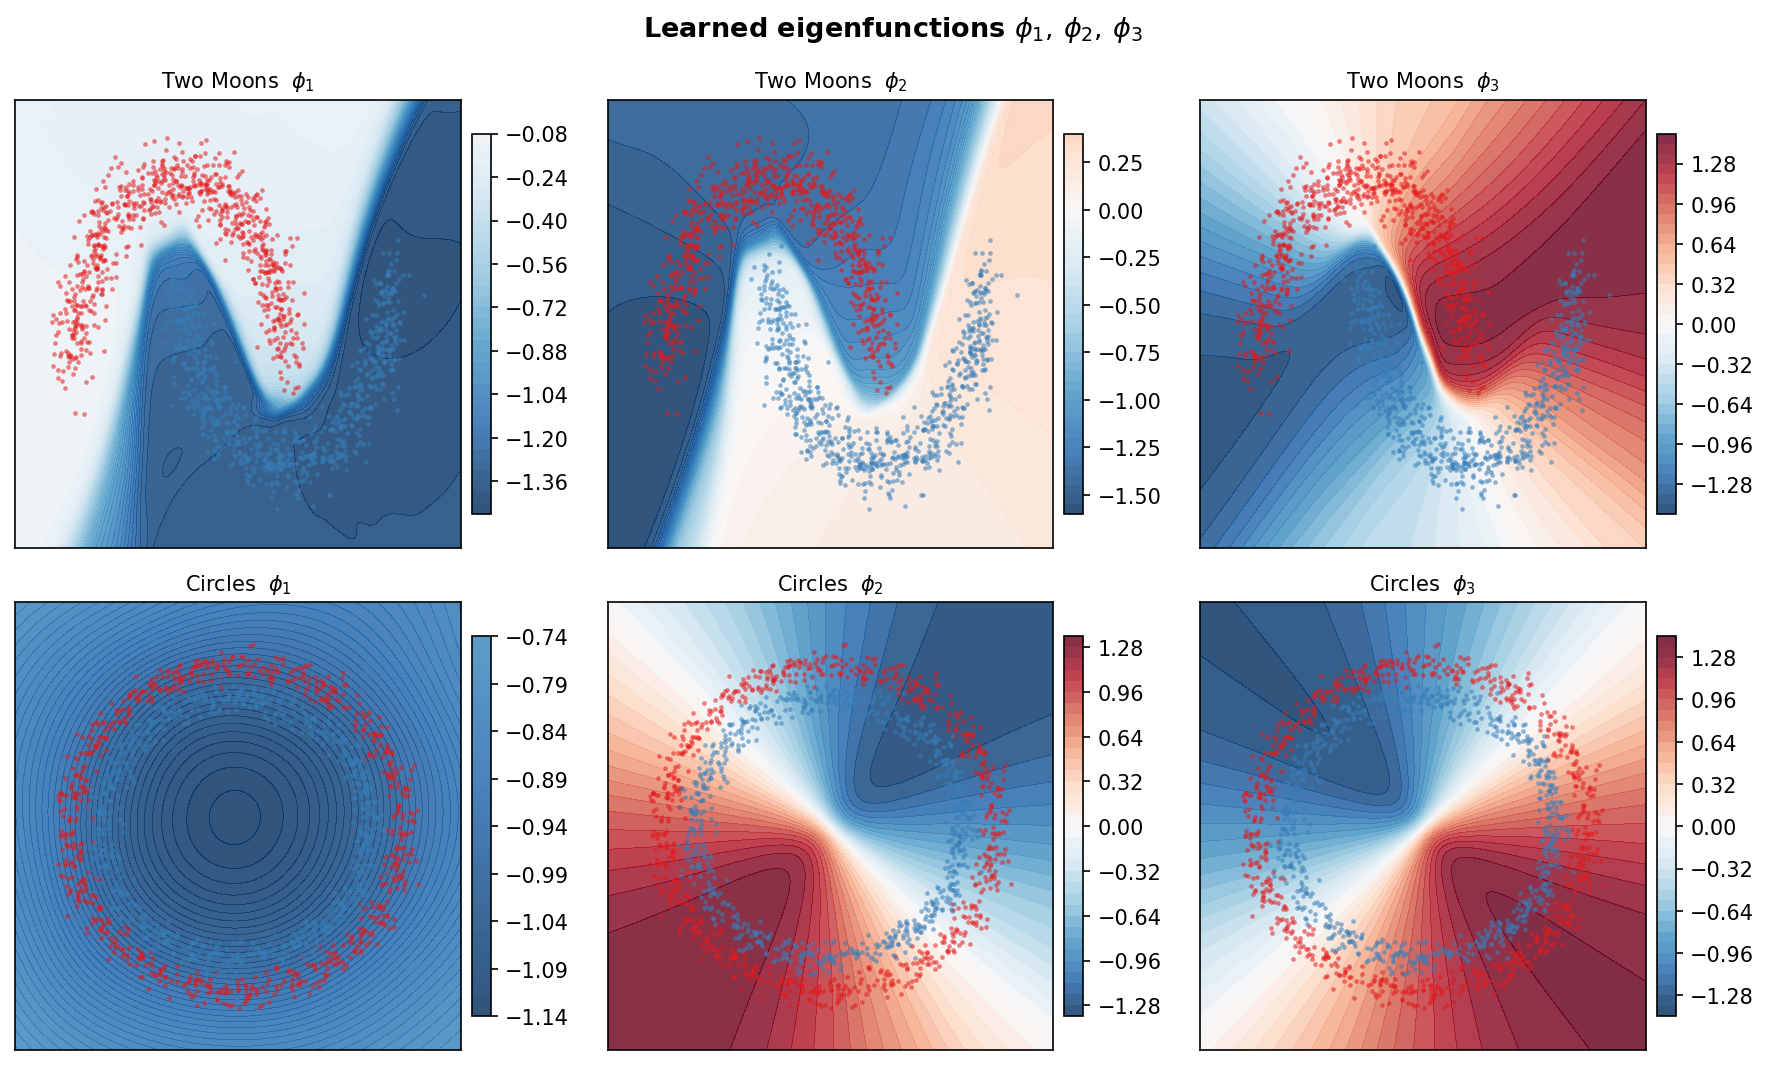
\includegraphics[width=\linewidth]{fig_eigenfunctions}
  \caption{\new{Learned eigenfunctions $\phi_1,\phi_2,\phi_3$ for Two Moons (top) and Circles (bottom).
           Red/blue dots: class labels. Colour scale: eigenfunction value.}}
  \label{fig:eigenfunctions}
\end{figure}

\subsection{Training Dynamics}

Figure~\ref{fig:training} shows validation accuracy over training steps for MNIST and CIFAR-10
(EFDO-off and EFDO-diag, mean $\pm$ std over 5 seeds).
Both variants converge rapidly in the first 15k steps and remain stable thereafter,
with negligible variance across seeds.
The diagonal metric consistently achieves slightly lower accuracy on MNIST while providing
a small but consistent improvement on Fashion-MNIST.

\begin{figure}[h]
  \centering
  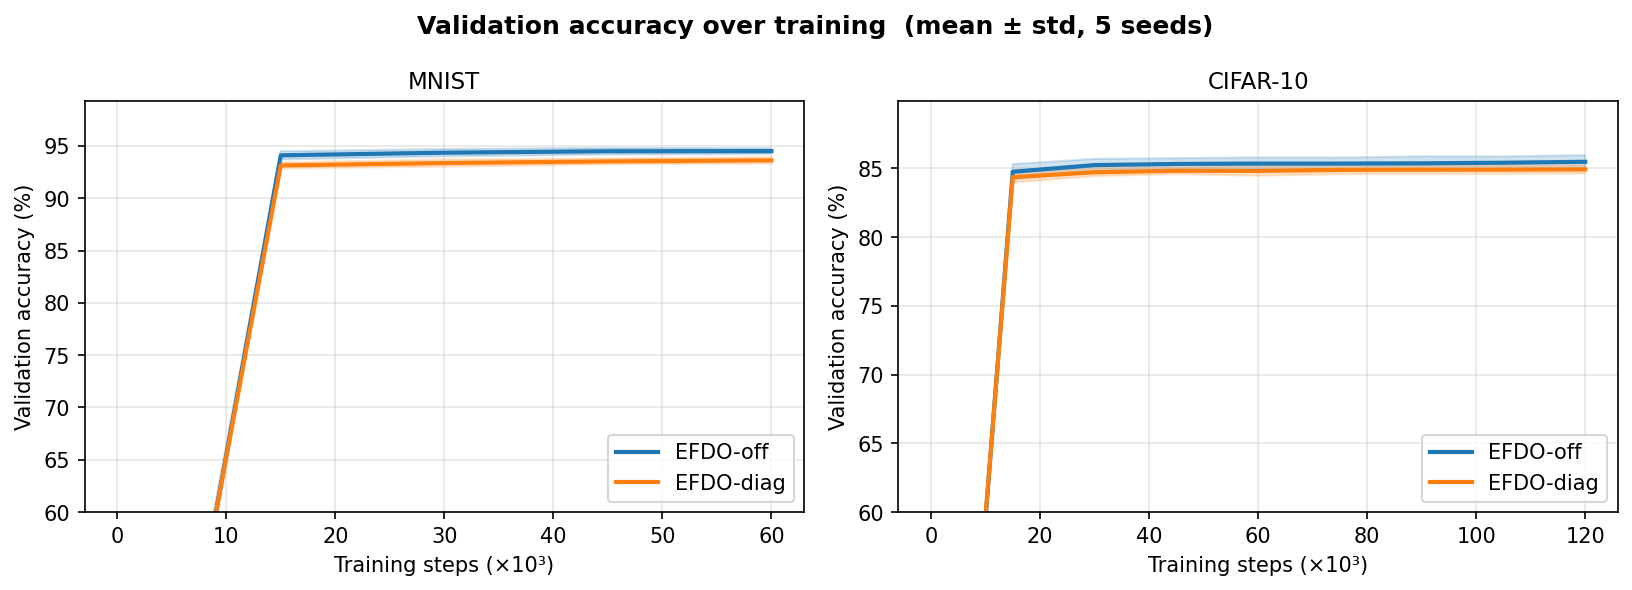
\includegraphics[width=\linewidth]{fig_training_curves}
  \caption{\new{Validation accuracy over training (mean\,$\pm$\,std, 5 seeds). Left: MNIST. Right: CIFAR-10.}}
  \label{fig:training}
\end{figure}

\subsection{Gram Matrix Analysis}

Figure~\ref{fig:gram} shows the Gram matrix $C_K = \mathbb{E}[\Phi\Phi^\top]$ computed on the
MNIST validation set after training (EFDO-off, $K{=}16$, seed 0).
The matrix is close to the identity, with Frobenius deviation $\|C{-}I\|_F < 0.5$ for the
first eigenfunctions, confirming that the orthonormality loss~\eqref{eq:loss_orth} successfully
enforces the constraint during sequential training.

\begin{figure}[h]
  \centering
  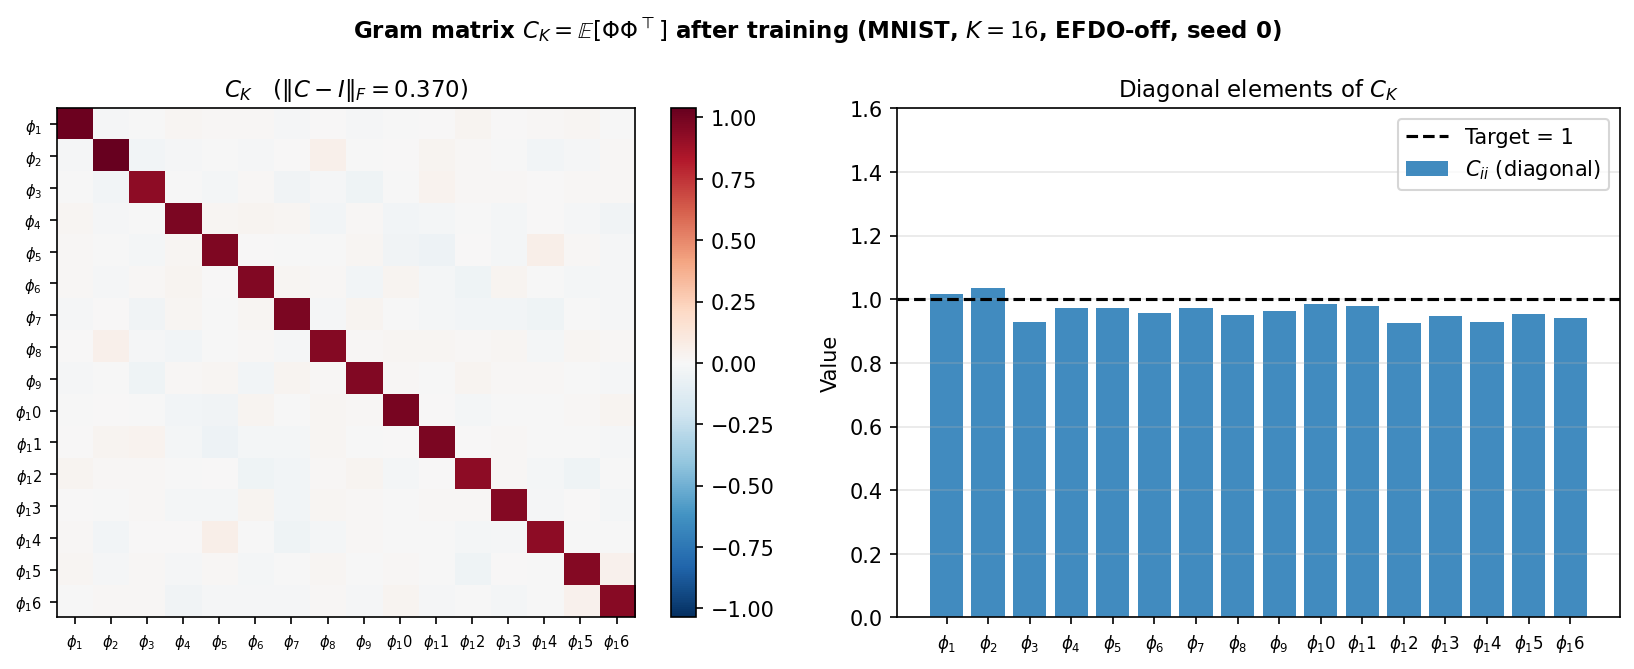
\includegraphics[width=\linewidth]{fig_gram_matrix}
  \caption{\new{Gram matrix $C_K$ (left) and diagonal elements (right) for MNIST EFDO-off, $K{=}16$, seed 0.
           Diagonal values close to 1 and small off-diagonal entries indicate near-orthonormal eigenfunctions.}}
  \label{fig:gram}
\end{figure}
}

We have performed all the simulations using PyTorch~\cite{NEURIPS2019_9015}
\new{on Google Colab A100 GPUs (multiclass datasets: MNIST, Fashion-MNIST, CIFAR-10)
and Apple M-series hardware (binary datasets).}
\new{Training time per seed: $\sim$2~min (Two Moons/HTRU2), $\sim$8~min (MNIST, 60k steps),
$\sim$25~min (CIFAR-10, 120k steps) on A100.}
Approximation of a single eigen-function takes about two hours \new{on CPU},
\new{and approximately 3--5 minutes per eigenfunction on GPU (MNIST, $d{=}784$)}.
Therefore, computational time is one of the most essential disadvantages of the proposed approach on CPU.
The solution to that problem could be appropriate initialization of the neural network,
but it is the subject of future research.

Finally, it is important to notice that the warm-up stage is critical to
avoiding local-minimum traps.
The intuition behind the weighting introduced is based on the observation that the Dirichlet Energy
is high for strongly oscillating functions. At the same moment, highly oscillating functions
are likely to have non-zero projection on the linear subspace of functions orthogonal to smooth eigenfunctions
that have been approximated already. Therefore, by promoting oscillations and orthogonality at the beginning of training,
we can increase the capability of ANN for detection of orthogonal directions in a function space.


\section{Discussion and Concluding Remarks.}
\label{sec:conclusion}
In the current work we present the novel sequential approach for approximation of Laplacian-like differential operators.
The central idea of the method is a two-stage procedure that allows the ANN to escape from the local minimum and
find the direction orthogonal to the space spanned by previously constructed eigenfunctions.
We achieve that by introducing the instability to the optimization process that deforms
the ANN approximation of eigen function to such a degree that novel direction can be discovered.

This instability stage or warm-up stage is followed by optimization of the loss function with positive weights with a certain hierarchy.
That weights are constructed in such a way that ANN tries to satisfy orthogonalization and normalization constraints first
before minimizing the objective function, which is the Dirichlet Energy.
This idea is quite generic and can be directly applied to training of other ANNs with constraints.

In addition to the novel ANN training algorithm, we study the problem of overfitting and ANN performance on outliers.
To address that issue, two data augmentation techniques have been proposed.
That regularization techniques can be considered as a perturbation of the probability distribution from which the data has
been sampled. The degree of that disturbance is adjusted in such a way that the disturbed probability distribution goes
to the original probability distribution as the number of samples goes to infinity.

Finally, we demonstrate on the datasets with different numbers of samples that the proposed approach for calculation
of eigenfunctions provides meaningful results at least from a machine learning point of view.
The accuracy of models trained on the eigenfunction values is similar to the accuracy of the models trained on the original data.
Moreover, in some cases training with eigenfunction values requires less samples to reach the similar accuracy in
comparison with training on the original data. Therefore, the presented approach can be adopted as a feature-engineering tool
for machine learning tasks. One of the main issues with the proposed approach is high computational cost.
However, it might be resolved with appropriate initialization strategy, which is a subject of future research.


\bibliography{bibliobase}
\bibliographystyle{icml2026}

%%%%%%%%%%%%%%%%%%%%%%%%%%%%%%%%%%%%%%%%%%%%%%%%%%%%%%%%%%%%%%%%%%%%%%%%%%%%%%%
%%%%%%%%%%%%%%%%%%%%%%%%%%%%%%%%%%%%%%%%%%%%%%%%%%%%%%%%%%%%%%%%%%%%%%%%%%%%%%%
% APPENDIX
%%%%%%%%%%%%%%%%%%%%%%%%%%%%%%%%%%%%%%%%%%%%%%%%%%%%%%%%%%%%%%%%%%%%%%%%%%%%%%%
%%%%%%%%%%%%%%%%%%%%%%%%%%%%%%%%%%%%%%%%%%%%%%%%%%%%%%%%%%%%%%%%%%%%%%%%%%%%%%%
\newpage
\appendix
\onecolumn
\section{You \emph{can} have an appendix here.}

You can have as much text here as you want. The main body must be at most $8$
pages long. For the final version, one more page can be added. If you want, you
can use an appendix like this one.

The $\mathtt{\backslash onecolumn}$ command above can be kept in place if you
prefer a one-column appendix, or can be removed if you prefer a two-column
appendix.  Apart from this possible change, the style (font size, spacing,
margins, page numbering, etc.) should be kept the same as the main body.
%%%%%%%%%%%%%%%%%%%%%%%%%%%%%%%%%%%%%%%%%%%%%%%%%%%%%%%%%%%%%%%%%%%%%%%%%%%%%%%
%%%%%%%%%%%%%%%%%%%%%%%%%%%%%%%%%%%%%%%%%%%%%%%%%%%%%%%%%%%%%%%%%%%%%%%%%%%%%%%

\end{document}

% This document was modified from the file originally made available by
% Pat Langley and Andrea Danyluk for ICML-2K. This version was created
% by Iain Murray in 2018, and modified by Alexandre Bouchard in
% 2019 and 2021 and by Csaba Szepesvari, Gang Niu and Sivan Sabato in 2022.
% Modified again in 2023 and 2024 by Sivan Sabato and Jonathan Scarlett.
% Previous contributors include Dan Roy, Lise Getoor and Tobias
% Scheffer, which was slightly modified from the 2010 version by
% Thorsten Joachims & Johannes Fuernkranz, slightly modified from the
% 2009 version by Kiri Wagstaff and Sam Roweis's 2008 version, which is
% slightly modified from Prasad Tadepalli's 2007 version which is a
% lightly changed version of the previous year's version by Andrew
% Moore, which was in turn edited from those of Kristian Kersting and
% Codrina Lauth. Alex Smola contributed to the algorithmic style files.
